\section{ICN-IoT Middleware Design}
In this section, we present the overall ICN-IoT middleware design. It consists of three system components, as shown in Figure~\ref{fig:phy} --  Embedded Device, Aggregator, Local Service Gateway, and IoT server, which offer five principle middleware functionalities, including device discovery, device naming service, IoT service discovery and Pub/Sub management.
%to develop IoT middleware over ICN network.
In contrast to centralized or overlay-based implementation in the legacy IP-based IoT platform, our ICN-IoT architecture pushes these middelware functionalities down to the distributed components to enable self-configuring subsystem to provide not only local services but can also scale to large IoT service.
%In legacy IP-based IoT platform, these functionalities are almost implemented on a centralized server, or over-lay application. In our ICN-IoT middleware architecture, they are pushed down to distributed components which can form a self-configuring subsystem to provide local service as well as a complete system that enables global communication.
\begin{figure}
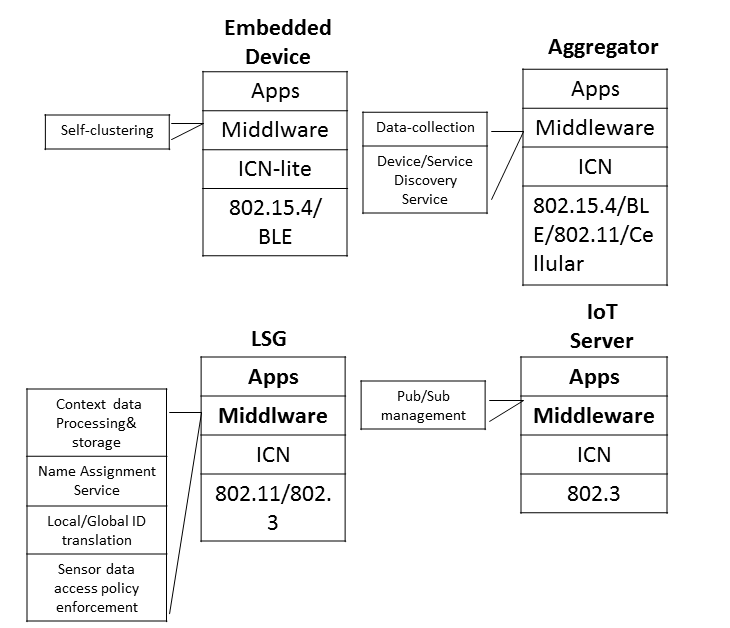
\includegraphics[width=\columnwidth]{figure/physical_comp.png}
\caption{\label{fig:phy}System Architecture of ICN-IoT middleware}
\end{figure}
\vspace{-1mm}
\subsection{System Architecture}\label{sec:physical}

The proposed architecture has the following four main system components:
\begin{itemize}
%\vspace{-2pt}
\item{\em Embedded Device}, which enables seamless ICN protocol in resource-constraint network. An ICN embedded device supports at least one of following communication mode: transmitting and routing over the data to the Aggregator, or responding the request based on name or ID.
\item{\em Aggregator}, which interconnects various IoT services and content in a local network. An Aggregator usually plays two roles: one is to act as the gateway to bridge the communication between resource-constrained wireless sensors and the rest of the nodes in the local network,  and the other one is to integrate sensing/actuating services in the local network.

%for resource-constraint wireless sensors, or it can be a device that integrates sensing/actuating service.

%\vspace{-2pt}
\item{\em Local Service Gateway (LSG)}, which connects the local IoT system to the rest of the global IoT system, and handles local name assignment and enforces  data access policies for local IoT devices. In addition, it can run context processing services to publish only the contextual information (instead of raw data) to the IoT server.
%It connects local IoT system to the outside world. It handles local name assignment and sensor data access policy enforcement. Furthermore, context data processing service can be implemented within this entity to publish only the information abstraction to IoT server.

%\vspace{-2pt}
\item{\em IoT Server}, which is a centralized server that maintains subscription memberships and provides the lookup service for subscribers. Unlike legacy IoT servers that are involved in the data path from publishers to subscribers -- raising the concern of its interfaces being a bottleneck -- the IoT server in our architecture is only involved in the control path where publishers and subscribers exchange their names and certificates.

%Legacy IoT server also involves in the data path from publisher to subscriber, where the bandwidth of its interfaces could be a bottleneck. In contrast, IoT server in our architecture only involves in control path in which publishers and subscribers exchange their names and certificates.
\end{itemize}

In the following subsections, we will discuss the functionality for each system component (as shown in Figure~\ref{fig:phy}) and present detailed protocol design considering NDN and MF.

\subsection{Device and Network Service Discovery}
Device discovery is a key component of any IoT system.  The objective
of device discovery is to expose new devices to the rest of the IoT
system -- every entity should be exposed to its direct upstream
device and possibly other devices.  Specifically, it includes the
following three aspects: (1) a newly-added sensor should be exposed
to its aggregator, and possibly to its LSG and the IoT server; (2) a
newly-added aggregator is exposed to its LSG, and possibly to its
neighbor aggregators; and (3) a newly-added LSG should be exposed to
the IoT server.  We note that device discovery could be used in other
contexts, such as neighboring sensors discovering each other to form
routing paths, but in this draft, we use the term to specifically
mean discovering new devices for IoT middleware purpose.

During device discovery for newly-added sensors, the sensor passes
its device-level information (such as manufacture ID and model
number) and application-level information (such as service type and
data type) to the upstream devices.  If the sensor is to have an ICN
name, the name is assigned by the naming service (described in
Section ~\ref{sec:naming}), and recorded by both the LSG and the aggregator (and possibly the IoT server).

ICN enables flexible and context-centric device discovery which is
important in IoT ecosystem where heterogeneous IoT systems belonging
to different IoT services may co-exist.  Contextualization is a
result of name-based networking where different IoT services can
agree on unique multicast names that can be pre-provisioned in end
devices and the network infrastructure using the routing control
plane.  This also has an advantage of localizing device discovery to
regions of network relevant to an ICN service, also enabling certain
level of IoT asset security.  In contrast IP offers no such natural
IoT service mapping; any forced mapping of this manner will entail
high configuration cost both in terms of device configuration, and
network control and forwarding overhead.

In the device discovery phase, sensors expose their information, such
as its manufacture secure ID and model name, to the upstream
aggregators pulling information from sensors.  There are two ways of
achieving this aim: (1) sensors pushing the information towards the
aggregators, and (2) aggregators pulling the information from
sensors.  In both NDN and MF, the pulling method is used.  In NDN,
this process is initiated by the configuration service running on LSG, which periodically broadcasts discovery Interests (using the
name /iot/model).The new sensor replies to the discovery interest
with its information, and the configuration service then registers
the sensor and generates a local ICN name for the sensor.  In MF, we
can set group-GUID as the destination address, and the configuration
service issues a request via multicasting.  When receiving such
request, the new device replies with the manufacture secure ID, and
the configuration service registers the device and generates a local
ICN name for it.

LSG, which periodically broadcasts discovery Interests (using the
name /iot/model).The new sensor replies to the discovery interest
with its information, and the configuration service then registers
the sensor and generates a local ICN name for the sensor.  In MF, we
can set group-GUID as the destination address, and the configuration
service issues a request via multicasting.  When receiving such
request, the new device replies with the manufacture secure ID, and
the configuration service registers the device and generates a local
ICN name for it.

The network service discovery for IoT infrastructure service like
naming, gateway, or context-processing service is hosted on LSGs or
Aggregators.  These devices periodically broadcast their services,
which will be responded to by sensors that need these services.
Please note that only those sensors that need naming service or
context processing service will respond.  The detailed process is
very similar to that involved in the device discovery (which is described above).

\iffalse
\begin{figure}
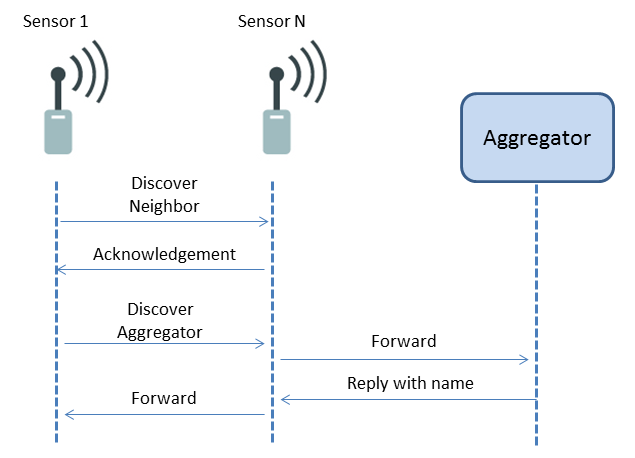
\includegraphics[width=\columnwidth]{figure/device_discovery.png}
\caption{\label{fig:device_dis}Device discovery for resource-constrained sensor}
\end{figure}
\fi


\subsection{Service Discovery}
Service discovery intends to learn IoT services that are hosted by
one aggregator by its neighbor aggregators.  The requirements include
low protocol overhead (including low latency and low control message
count), and discovery accuracy.

In today's IoT platforms, sensors, aggregators and LSGs are connected
via IP multicast, which involves complicated group management and
multicast name to IP translation service.  Multicast, however, is
greatly simplified in ICN as most ICN architectures have natural
support for multicast.

Below, we explain how service discovery is implemented.  The key to
service discovery is to expose aggregator's services to its neighbor
aggregators.  How this is implemented differs in NDN and MF.  In NDN,
the source aggregator broadcasts an interest using the well-known
name $/area/servicename/certificate$, which will eventually reach the
destination aggregator.  NDN's Interest/Data mechanisms allows only
one response for each Interest send while discovery requires to learn
multiple entities, hence efficient discovery is realized using
exclusion via Selectors in the protocol or as an overlay protocol~\cite{ravindran2013information}.

In MF, after establishing the multicast group, the source aggregator sends a
request containing the service name and certificate to the multicast
group.  The destination aggregator that hosts the service checks the
certificate and registers the source Aggregator if there is a matched
service.  It replies with an acknowledgment containing certificate to
the source aggregator.

For secure service discovery, a secured name needs to assigned to the
service host.  Especially in MF IoT, secured group GUID is utilized
to realize service request multicast, which may be owned by multiple
hosts, hence conventional public/private key scheme may not be
suitable for this case.  As an alternative, group key management
protocol (GKMP) ~\cite{harney1997group} can be adopted to resolved the issue above -- A
naming service residing at LSG or IoT server (depending on
application scope) generates a group public key that used as group
GUID for a service, then this group public/private keys pair is
assigned to each Aggregator that host this service.  The service host
Aggregator in the group then listen on this group GUID, and use the
group private key to decrypt the incoming discovery message.
Finally, we note that this form of secure service discovery is
difficult for NDN.

As an example of NDN smart home, a thermostat expresses a request to
discover a AC service using well-known name $/home/ac/certificate$ via
broadcast channel.  In MF case, a multicast group GUID 1234 can be
assigned to all home appliance IoT service.  The thermostat sends
request containing the service name and certificate to 1234.  In both
cases, the AC hosting this services replies with acknowledgment if
all conditions match.
\begin{figure}
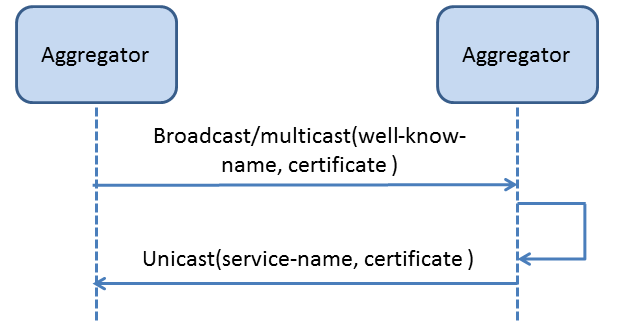
\includegraphics[width=\columnwidth]{figure/service_discovery.png}
\caption{\label{fig:ser_dis}General service discovery message flow for NDN and MF}
\end{figure}
\vspace{-1mm}
\iffalse
IoT services can be generally categorized into two classes: sensing and actuating. In today's IP based IoT platforms, sensors are connected via a server, which requires considerable development effort such as maintaining a local name to IP mapping. In ICN-IoT, IoT service discovery and configuration becomes much simpler. Specifically, we consider two service discovery modes: $peer$-$to$-$peer$ and $master$-$slave$.


\vspace{1mm}\noindent{\bf Peer-to-peer Service Discovery}: In this mode, we consider the scenario in which an aggregator (referred to as the source aggregator) tries to discover an IoT service provided by another peer aggregator (referred to as destination aggregator). In NDN, the source aggregator broadcasts an interest using the well-known name $/area/servicename/certificate$, which will eventually reach the destination aggregator. NDN's Interest/Data mechanisms allows only one response for each Interest send while discovery requires to learn multiple entities, hence efficient discovery is realized by using exclusion via Selector in the protocol or as an overlay protocol~\cite{ravindran2013information}. In MF, this is handled by multicast (discussed in Section~\ref{sec:intro_mf}) instead of flooding the entire local network. All sensors that provide relevant services can join the multicast group identified by a $Group$-$GUID$. After establishing the multicast group, the source aggregator sends a request containing the service name and certificate to the multicast group.The destination aggregator that hosts the service checks the certificate and registers the source Aggregator if there is a matched service. It replies with an acknowledgement containing its certificate to the source aggregator. The message flow is shown as Figure~\ref{fig:ser_dis}.

For an example of NDN smart home, a thermostat expresses a request to discover the air conditioning (AC) service using well-known name $/home/ac/certificate$ via broadcast channel. In MF case, a multicast group GUID $1234$ can be assigned to all home appliance IoT service. The thermostat sends request containing the service name and certificate to $1234$. In both cases, the AC hosting this services replies with acknowledgement if all conditions match.

\vspace{1mm}\noindent{\bf Master-slave Service Discovery}: In some IoT applications, there are more than one sensing service or actuating service connecting to one control service. A source aggregator hosting control service expresses a request with the service name and the  certificate to discover a service from all  available aggregators. By verifying the certificate, the destination aggregators  register the source aggregator and  answer with acknowledgement containing their certificates if the certificate is valid and there exists a matched service.

In the AC control NDN example, the number of AC service provider increases to three, which can be named as $/office/ac/1$, $/office/ac/2$ and $/office/ac/3$ . The thermostat expresses a partial name $/office/ac/certificate$ via a broadcast channel periodically. In the MF case, a multicast group GUID $1234$ can be assigned to identify AC service. The thermostat sends request with service name and certificate to $1234$. The destination ACs reply with their certificates if the request meets all criteria.
\fi

\subsection{Data Aggregation and Context Data Processing}
In order to facilitate context-aware communication and data
retrieval, we need to support context processing in the IoT system.
The objective of context processing is to expose the sensor's low-
level context information to upstream aggregators and LSGs, as well
as to resolve the application's high-level context requirements using
lower-level sensor contexts.  The context processing service usually
runs on both aggregators and LSGs.

Context processing requires the underlying network to be able to
support in-network computing at both application and network levels.
ICN inherently supports in-networking computing and caching, which
thus offers unique advantages compared to traditional IP network
where the support for in-network computing and caching is poor.

Application level contexts differ from application to application,
and therefore, we need to provide a set of basic mechanisms to
support efficient context processing.  Firstly, the network needs to
define a basic set of contextual attributes for devices (including
sensors, aggregators, and LSGs), including device-level attributes
(such as location, data type, battery level, etc), network-level
attributes (such as ICN names), and service-level attributes (such as
max, min, average, etc).

Secondly, we need to have means to expose sensor/aggregator/LSG
contextual attributes to the rest of the system, through centralized
services such as naming resolution service.

Thirdly, the IoT server needs to allow applications (either producers
or consumers) to specify their contextual requirements.  Fourthly,
the unconstrained part of ICN-IoT needs to be able to map the higher-
level application-specific contextual requirements to lower-level
device-level and network-level contextual information.


\subsection{Device/App Naming service}\label{sec:naming}
The objective of the naming service is to assure that either device
or service itself is authenticated, attempting to prevent sybil (or
spoofing) attack~\cite{sybil} and that the assigned name closely binds to the
device (or service).  Naming service is specific to MobilityFirst,
and it is hard to achieve in the context of NDN.  Naming service
assigns and authenticates sensor and device names.  An effective
naming service should be secure, persistent, and able to support a
large number of application agnostic names.

Traditional IoT systems use IP addresses as names, which are insecure
and non-persistant.  IP addresses also have relatively poor
scalability, due to its fixed structure.  Instead, ICN separates
names from locators, and assigns unique and persistent names to each
sensor/device, which satisfies the above requirements.

In what follows, we discuss an approach for secure naming service in
ICN-IoT.  We first consider the case where the embedded system is
programmable so that before deployment, the owner can preload
identity information (such as secure ID, a pair of public/private key
and a certificate) , or has some manufacture ID and a pair of public
private key (which is certified by the manufacturer).  That is, the
device is associated with information including device identity,
public/private keys ($PK_{device}$, $SK_{device}$) and a certificate
either from the owner or the manufacturer which certifies the device
identity and public/private keys.  When such a device is discovered,
the aggregator will first verify the device identity (e.g., the
device can generate a signature with the private key $SK_{device}$ and
present the signature and the certificate to the aggregator so that
the aggregator can verify it), and then assign a name to the device
as follows: the aggregator will issue a request to LSG together with
its device identity and $PK_{device}$, so that LSG can assign an NDN
name and generate a certificate (certifying the binding of NDN name,
$PK_{device}$).  To this end, the ICN name and the certificate will be
sent back to the aggregator and will be stored locally if the device
is resource-restricted.  Otherwise, the ICN name and the certificate
will be passed to the device.

For the MF-IoT, assigning a GUID for a device is rather
straightforward: after verifying the device identity, the Aggregator
inserts the public key $PK_{device}$ and device information to the
upper layer component to verify if there is a conflict in the
corresponding scope.  Specifically, LSG is in charge of local scope
and IoT server guarantees the global uniqueness.  Finally, the unique
public key is used a GUID for the new device.  Analogously, service
discovery can be secured in a similar way.

In the case where devices are only associated with the secure
manufacture ID while without being pre-loaded public/private keys and
the certificate, it is critical to assure that devices are
authenticated by using other trust model.  For example the system can
take advantage of the web-of-trust model or the contextually semantic
information so that the devices manufactured by the same vendor can
authenticate each other.  Moreover, in order to comply with the
capability of resource-restricted devices, light-weight cryptographic
primitive (such as symmetric cryptography) may be used instead of
public key cryptography.

Finally, we note that the same naming mechanism can be used to name
higher-level IoT devices such as aggregators and LSGs.


\subsection{Publish/Subscribe Management}
Data Publish/Subscribe (Pub/Sub) is an important function for ICN-IoT, and is responsible for IoT information resource sharing and management. The objective of pub/sub system is to provide centralized membership management service. Efficient pub/sub management poses two main requirements to the underlying system: high data availability and low network bandwidth consumption.

In conventional IP network, most of the IoT platforms provide a centralized server to aggregate all IoT service and data. While this centralized architecture ensures high availability, it scales poorly and has high bandwidth consumption due to high volume of control/data exchange, and poor support of multicast.

Next we consider two decentralized pub/sub models.  The first one is the Rendezvous mode that is commonly used for today's pub/sub servers, and the second one involves Data-Control separation that is unique to ICN networks where the control messages are handled by the centralized IoT server and the data messages are handled by the underlying ICN network.  Compared to the popular Rendezvous mode where both control and data messages both meet at the centralized
server, separating data and control messages can greatly improve the scalability of the entire system, which is enabled by the ICN network.

In today's IP network, Rendezvous mode is the classic pub/sub scheme in which data and requests meet at an intermediate node.  In this case the role of the IoT server is only required to authenticate the consumers and providing it Rendezvous service ID.

While NDN is a Pull-based architecture without supporting the Pub/Sub mode naturally,  COPSS~\cite{chen2011copss} proposes a solution to fix this problem. It integrates a Push-based multicast feature with the pull based NDN architecture at the network layer by introducing Rendezvous Node (RN). RN is a logical entity that resides in NDN forwarder. The publisher first forwards a Content Descriptor (CD) as a snapshot to the RN. RN maintains a subscription table, and receives the Subscription message from subscribers. The data publisher just sends the content using Publish packet by looking up FIB instead of PIT. If the same content prefix is requested by multiple subscribers, RN will deliver one copy  of content downstream, which reduces the bandwidth consumption substantially.

\begin{figure}
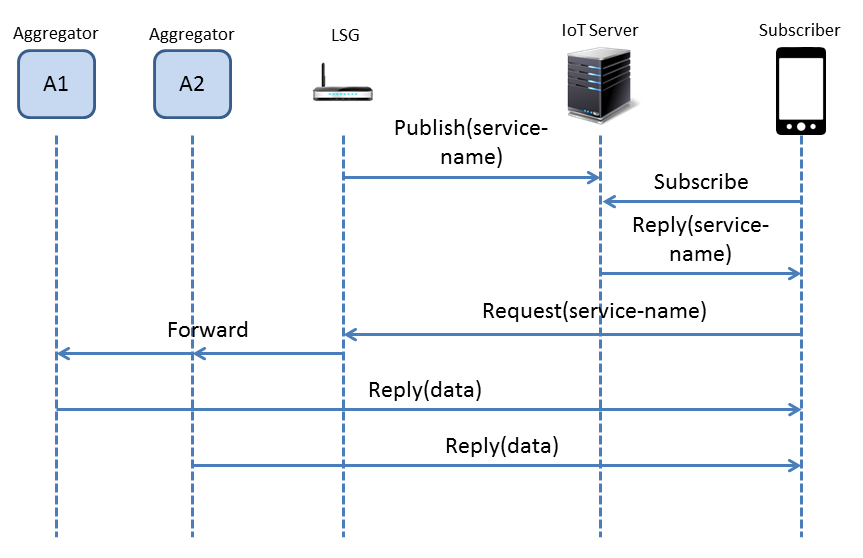
\includegraphics[width=\columnwidth]{figure/pub_sub.png}
\caption{\label{fig:pubsub}Publish/subscriber management message flow}
\end{figure}

Compared with the Rendezvous mode in which data plane and control plane both reside on the same ICN network layer, we consider an architecture where the control message is handled by the centralized server while data is handled by ICN network layer.  Following the naming process mentioned above, the LSG has the ICN name for the local resource which is available for publishing on IoT server.  IoT server maintains the subscription membership, and receives subscription requests from subscribers. Since the subscribers has non knowledge about the number of resource providers and their identities  in a dynamic scenario,  IoT server has to take responsibility of grouping and assigning group name for the resource. The generic message flow for publish/subscribe function is shown in Figure~\ref{fig:pubsub}, and we will illustrate the detail for NDN and MF.
In NDN, the grouping resource is intuitive: all resources have the same schematic prefix will be grouped together, and the prefix can be used to identify the service. The traditional NDN supports using a common partial name to retrieve multiple resources via Selector, but M. Amadeo et al. ~\cite{amadeo2014multi} provides a more efficient solution to improve this mechanism by introducing long-life multi-source Interest in PIT. MF takes advantage of  $Group$-$GUID$ to identify a service provided by multiple resources. This $Group$-$GUID$ will be distributed to the subscriber as well as the publisher. In an example of NDN,  it uses the common prefix$/home/monitoring/$ to identify a group of resource that provides multiple monitoring services such as $/home/monitoring/temperature$ and $/home/monitoring/light$. The subscriber retrieves the prefix from the IoT server, and sends Interest toward the resource. In a MF example, $GUID$-$x$ identifies the ``home monitoring'' service that combines with ``light status'' and ``temperature''. The resource producers, i.e. the host of ``temperature'' and the host of ``light status'' are notified that their services belong to $GUID$-$x$, then listen on $GUID$-$x$. The subscriber sends the request containing  $GUID$-$x$ through multicasting which ultimately reaches the producers at last common node. Once receiving the request, the resource producer unicasts the data to the subscriber. In addition, if multiple resource consumers subscribe to the same resource, the idea of $Group$-$GUID$ can be reused here to group the consumers to further save bandwidth using multicast.

